\documentclass[protokol.tex]{subfiles}
\begin{document}
Podmínky měření jsou uvedeny v následující tabulce.
\begin{table}[H] \label{tab:podminky}
\centering
\setlength{\tabcolsep}{10pt}
\begin{tabular}{ccc}                                                    \toprule
Teplota                 &   Tlak                    &   Vlhkost     \\
$[\si{\degreeCelsius}]$ &   $[\si{\hecto\pascal}]$  &   [\% RH]     \\  \midrule
25,3                    &   984,5                   &   29,8        \\  \bottomrule
\end{tabular}
\caption{Podmínky měření}
\end{table}

Všechny délkové rozměry byly měřeny mikrometrem. Rozměry vzorku před deformací:
$$ l_0 = (10,03 \pm 0,01) \ \si{\milli\metre} $$
$$ d_0 = ( 7,43 \pm 0,01) \ \si{\milli\metre} $$
Rozměry po deformaci:
$$ l = ( 9,88 \pm 0,01) \ \si{\milli\metre} $$
$$ d = ( 7,47 \pm 0,01) \ \si{\milli\metre} $$


Data naměřená v rámci zjišťování tuhosti aparatury jsou vynesena v přiloženém grafu 1. Použitý vzorek považujeme za absolutně tuhý.

Data naměřená při dynamické zkoušce deformace vzorku jsou vynesena v přiloženém grafu 2.
\subsection*{Úkol 1}
Tuhost aparatury určíme fitem lineární části závislosti \eqref{eq:tuhost} v přiloženém pracovním grafu 3 rovnicí $f(x) = K x + b$.
$$ K = (1839,7 \pm 0,5) \times 10^3 \ \si{\newton\per\metre}. $$

\subsection*{Úkol 3}
Veličiny byly přepočítány podle postupu popsaném v teorii, pro lineární regresi byla vybrána oblast dat s lineárním průběhem.
\begin{figure}[H]
\centering
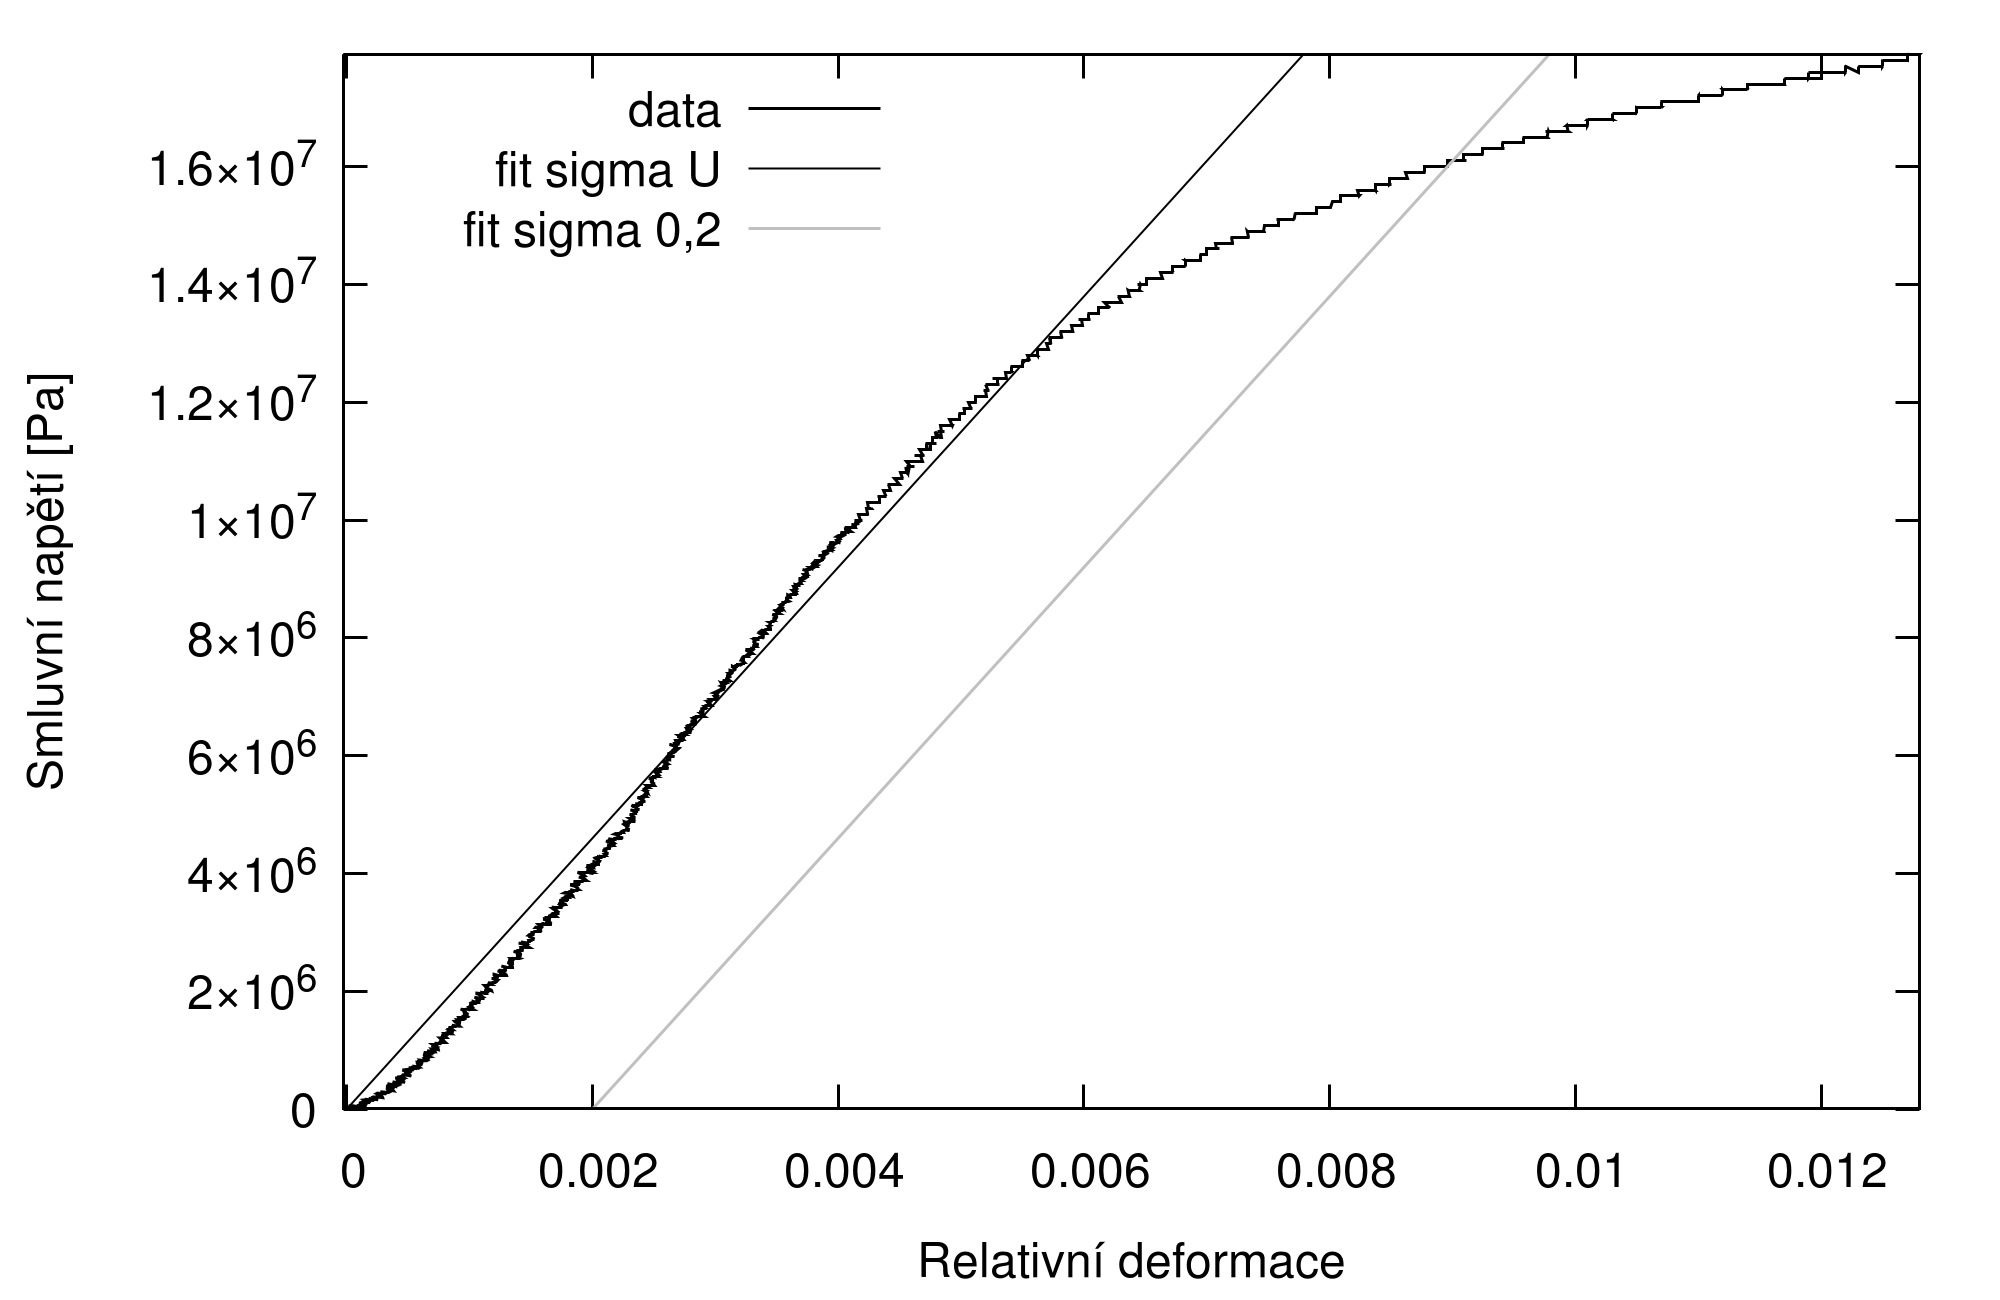
\includegraphics[resolution=350]{plot/graf}
\caption{Graf závislosti napětí na relativním prodloužení}
\end{figure}
Z lineární regrese v grafu určíme $\sigma_U$ a $\sigma_{0,2}$. Chyby těchto hodnot jsou určené odhadem.
$$ \sigma_U = (1,3 \pm 0,1) \times 10^7 \ \si{\pascal} $$
$$ \sigma_{0,2} = (1,6 \pm 0,1) \times 10^7 \ \si{\pascal} $$
\end{document}
